\chapter{Modelling} \label{chp:models}
    

    \section{Absorption}
        A critical property of LSP is its ability to absorb laser radiation. As stated in \autoref{sec:background_lsp}, the primary mechanism for radiation absorption in LSP is inverse-brehmsstrahlung. Calculation of the absorption coefficient of this process is critical for modelling LSP behavior and estimating its laser absorption efficiency. The calculation method presented here aims to adapt the work of \textcite{akarapuNumericalModelLasersustained2009,nassarInvestigationLasersustainedPlasma2012}, who have developed CFD models for the use of Argon LSP in surface-treatment applications. Although their work considered \ce{CO_2} lasers, adapting the method to the fiber laser of this study is a matter of using the appropriate laser frequency in \autoref{eq:ib_absorption}. Their work was thus used to validate each calculation step, and their results will often be plotted against this study's computations when relevant.
        
        The absorption coefficient can be calculated using \autoref{eq:ib_absorption}, and is heavily-dependent on electron density $n_\mathrm{e}$ and radiation frequency $\nu$. The first step of absorption modelling is thus to determine electron density, which is variable with temperature $T$ according to the Saha ionization equation, developed by \textcite{sahaPhysicalTheoryStellar1997}. It is reproduced here for the single-ionization case as \autoref{eq:saha}:
        \begin{equation}
            \frac{n_\mathrm{e}^2}{n_0-n_\mathrm{e}} = \frac{n_\mathrm{e}^2}{n_\mathrm{Ar}} = \frac{2}{\Lambda_\mathrm{th}^3}\frac{Z_{\mathrm{Ar}^+}}{Z_\mathrm{Ar}}\exp{\left(-\frac{E_\text{ion, Ar}}{k_\mathrm{B}T}\right)}
            \label{eq:saha}
        \end{equation}
        Where $n_0$ is the initial number density of neutral atoms, $n_\mathrm{Ar}$ is the number density of un-ionized atoms at a given temperature, $E_\text{ion, Ar}$ is Argon's first ionization energy (\qty{15.76}{eV}), and $k_\mathrm{B}$ is the Boltzmann constant. The thermal DeBroglie wavelength $\Lambda_\mathrm{th}$ is a function of temperature as follows, where $\hbar$ is the reduced Planck constant and $m_\mathrm{e}$ is the mass of an electron:
        \begin{equation*}
            \Lambda_\mathrm{th} = \sqrt{\frac{2\pi \hbar^2}{m_\mathrm{e}k_\mathrm{B}T}}
        \end{equation*}
        The ratio $Z_{\mathrm{Ar}^+}/Z_\mathrm{Ar}$ is the ratio of the partition function values for Ar$^+$ and Ar (also designated Ar II and Ar I, respectively). These values are also dependent on temperature and can be queried in the NIST Atomic Spectra Database (\textcite{kramidaNISTAtomicSpectra2022}) for a given spectrum (e.g., Ar I) and electron temperature $T_\mathrm{e}$. This ratio is plotted in \autoref{fig:e_density_partition}. \citeauthor{nassarInvestigationLasersustainedPlasma2012} fitted a seventh-order polynomial to approximate this ratio across temperature, which is also plotted for comparison.

        It is important to note that $n_0$ in \autoref{eq:saha} is not constant across temperatures. In the case of LSP, the ionization process occurs at constant pressure, even if the experiment occurs in a closed container, as only a small fraction of the test-section volume undergoes ionization. The hotter Argon is free to expand into the cooler surroundings, locally reducing the number density and maintaining a constant pressure. Therefore, $n_0$ must be calculated based on a given pressure $p$ and the varying temperature. This can be done with the ideal gas equation, where $V$ is volume, $N$ is the number of atoms in moles, $R_\mathrm{u}$ is the universal gas constant, and $N_\mathrm{A}$ is Avogadro's number:
        \begin{align*}
            pV&= NR_\mathrm{u}T \\
            p&= \frac{N}{V}R_\mathrm{u}T \\
            \frac{N_\mathrm{A}p}{R_\mathrm{u}T}&= n_0
        \end{align*}

        The electron density $n_\mathrm{e}$ is plotted against temperature in \autoref{fig:e_density_curves}, for a pressure of \qty{1}{bar}. The calculation by \citeauthor{nassarInvestigationLasersustainedPlasma2012} is plotted alongside it, and their relative value is compared. While the electron density plots appear to agree, there remains a difference of density of a factor 2. This appears to be due to the use of lower precision physical constants in \citeauthor{akarapuNumericalModelLasersustained2009} and \citeauthor{nassarInvestigationLasersustainedPlasma2012}'s work.

        \begin{figure}[h]
            \centering
            \begin{subfigure}[t]{2.6in}
                \centering
                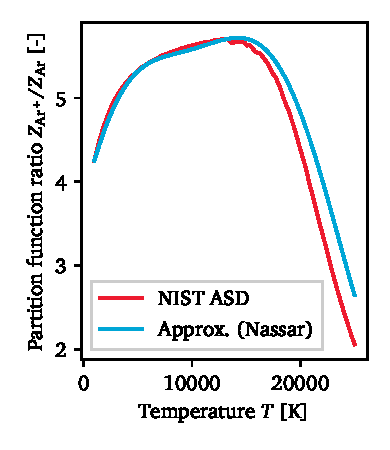
\includegraphics[]{assets/4 models/partition}
                \caption{Ratio of Ar II to Ar I partition function values}
                \label{fig:e_density_partition}
            \end{subfigure}
            \hfill
            \begin{subfigure}[t]{3.2in}
                \centering
                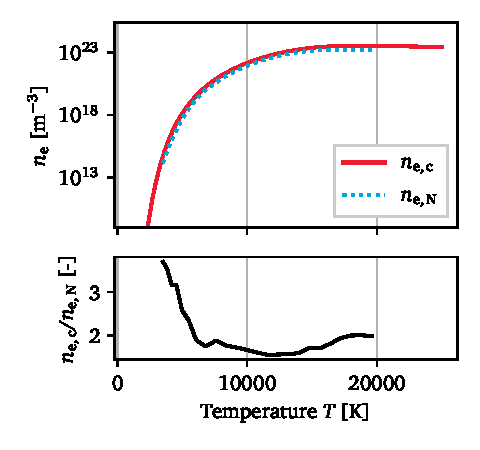
\includegraphics[]{assets/4 models/n_e}
                \caption{$n_e$ at \qty{1}{bar}, and comparison between computed density $n_\mathrm{e, c}$ and density $n_\mathrm{e, N}$ reported by \textcite{nassarInvestigationLasersustainedPlasma2012}}
                \label{fig:e_density_curves}
            \end{subfigure}
            \caption{Computation of electron density $n_e$ of Argon}
            \label{fig:e_density}
        \end{figure}

        \begin{figure}[h]
            \centering
            \begin{subfigure}[t]{2.9in}
                \centering
                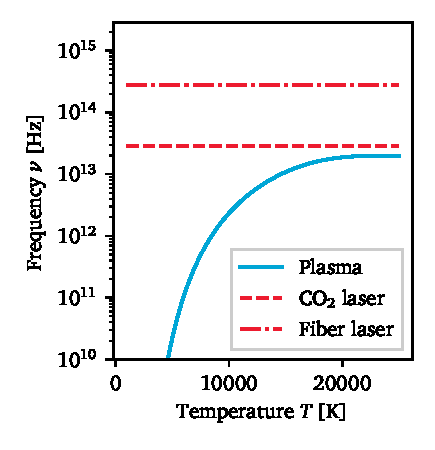
\includegraphics[]{assets/4 models/frequency_comparison}
                \caption{Comparison of plasma frequency to laser frequency, \qty{10}{bar}}
                \label{fig:coulomb_freq}
            \end{subfigure}
            \hfill
            \begin{subfigure}[t]{2.9in}
                \centering
                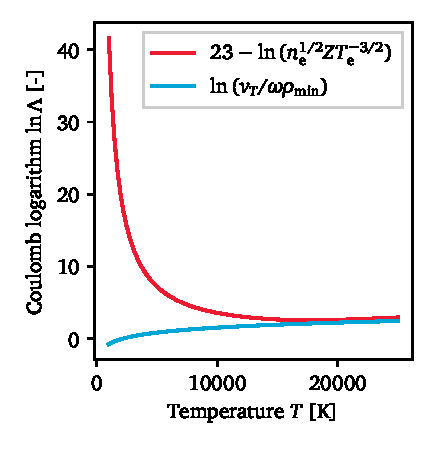
\includegraphics[]{assets/4 models/coulombLog}
                \caption{Comparison of computation methods for the Coulomb logarithm}
                \label{fig:coulomb_coulomb}
            \end{subfigure}
            \caption{Calculation of the Coulomb logarithm}
            \label{fig:coulomb}
        \end{figure}

        \begin{figure}[h]
            \centering
            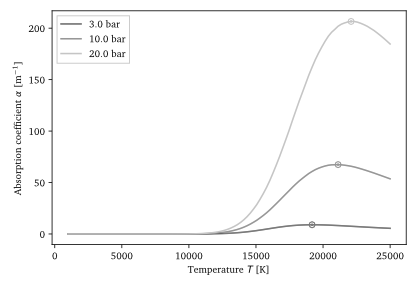
\includegraphics[]{assets/4 models/absorption}
            \caption{Inverse-brehmsstrahlung absorption coefficient of Argon at various pressures}
            \label{fig:ib_coeff}
        \end{figure}